
\chapter{Systemarkitektur}
\begin{longtabu} to \linewidth{@{}l l l X[l]@{}}
	
	
	Version &    Dato &    Ansvarlig &    Beskrivelse\\[-1ex]
	\midrule
	0.1 &    03-11-2015 &    MB &    Oprettelse \\[-1ex]
	0.2 &    10-11-2015 &    DHC, MB &     HW Start af skrivning, indsætning af billeder  \\[-1ex]
	0.3 &  11-11-2015   &  DHC   &   HW Design Forstrækning  \\[-1ex]
	0.4 & 18-11-2015 & ABH & HW Rettelse af diagrammer \\[-1ex]
	0.5 & 18-11-2015 & DHC, AJF & HW Implementering Forstrækning, Modultest Lavpas \\ [-1ex]
	0.6 & 18-11-2015 & ABH & SW Design, Metodeidentifikation \\[-1ex]
	0.7 & 26-11-2015 & DHC & HW Modultest, Kalibrering ved vandsøjle \\ [-1ex]
	0.8 & 26-11-2015 & DHC, AJF & HW Design Lavpas \\ [-1ex] 
	
	\label{version_Systemark}
\end{longtabu}

I det følgende beskrives arkitekturen for systemet. Systemarkitekturen er vores udviklingsramme for den videreudvikling af design og implementering af blodtrykssystemet. Designet af systemet er grebet an således at der først kigges på det overordnede system, hvorefter systemet arbejdes ned i mindre brudstykker. Dette gøres ved at benytte diagrammer med tilhørende beskrivelser.

\section{Hardware}
\subsection{Design}

Systemets hardware kan illustreres i et BBD. Det ses at nedenstående figur at systemet består af fem hardware blokke: software system, forstærker, filter, DAQ og transducer. Disse fem blokke udgør til sammen selve blodtryksmåleren.  
	
\begin{figure}[H]
	\centering
	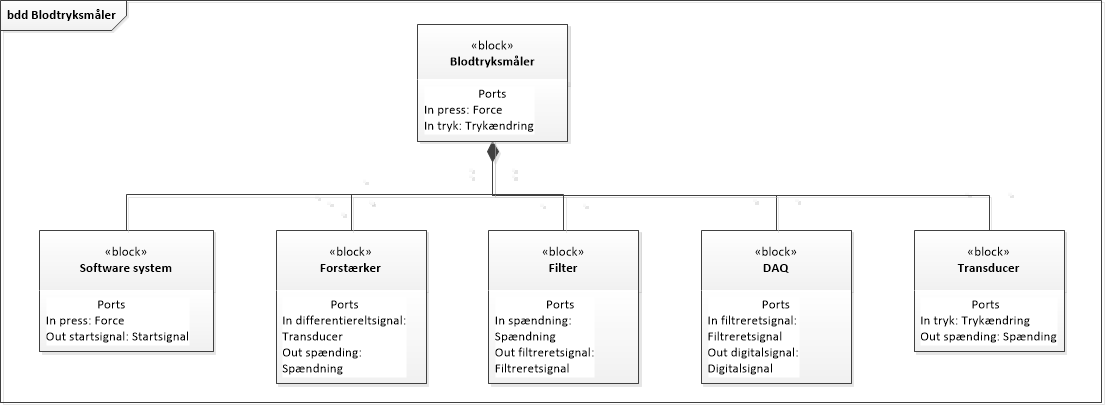
\includegraphics[width=1.0\textwidth]{Figurer/BDD}
	\caption{Block Definition Diagram for hardware}
	%\label{fig:BDD viser blodtrykssystemets hardwaredele, samt sammenhængen mellem disse}
\end{figure}

Ovenstående BDD-diagram fører videre til udarbejdelsen af IBD for hardware komponenterne. I dette diagram vises koblingen mellem de forskellige blokke gennem port forbindelser.  Det ses at signalet starter ved transduceren, hvorefter det bliver behandlet gennem forstærker, filter og DAQ. Til sidste sendes det ind i software systemet, som bliver påvirket af tryk på knapper på GUI. 

\begin{figure}[H]
	\centering
	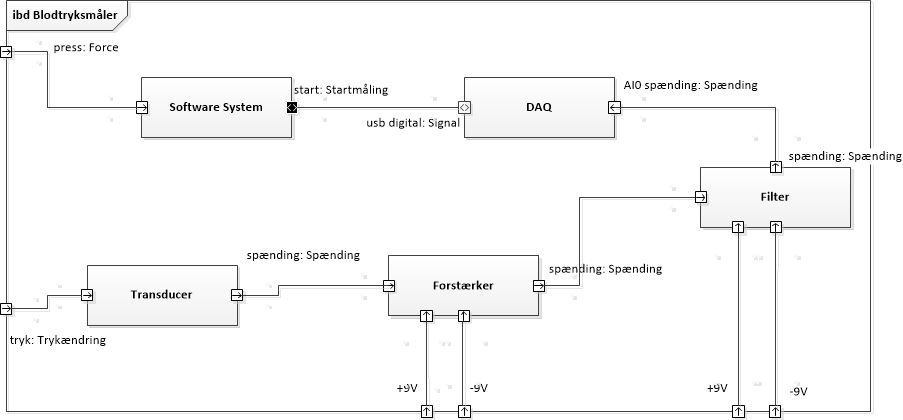
\includegraphics[width=1.0\textwidth]{Figurer/IBD}
	\caption{Infernal Block Diagram for hardware}
	\label{fig:IBD viser koblingen mellem blodtrykssystemets hardwaredele}
\end{figure}

\subsubsection{Forstærkning}
Transduceren måler en trykændring som den omsætter til en spænding. Dette er udtrykt ved et differentieret signal, som sendes ind i forstærkning-blokken. Da signalet fra transduceren er en lav spænding, skal det forstærkes op, for at det passer med DAQ'ens input. Denne forstærkning skal udregnes ud fra det maksimale output fra transduceren og det maksimale input til DAQ'en. Se under Implementering.  

Under simulering bruges Analog Discovery som en funktionsgenerator, der simulere det differentieret signal. Analog Discovery har en usikkerhed, når der arbejdes med små spændinger. Dette kan modarbejdes vha. spændingsdeler princippet. Dette gør at Analog Discovery kan sende en højere spænding ind i systemet, så usikkerheden mindskes.  

\subsubsection{Lavpas}
I projektet skal der laves et 2. ordens lavpasfilter. Filteret skal laves for at sikre, at der ikke opstår aliasering. Det sikre derfor at der ikke er noget signal ved den halve samplingsfrekvens.\\
Aliasering  REFERENCE (DSB-bogen)er, hvor signalet bliver gentaget. Når man har signalet i det digitale domæne, bliver spektret for signalet en periodisk funktion. Det vil sige, at den gentager sig selv, efter et bestemt stykke tid. \\
Det skal sikres, at der ikke kommer overlap mellem signalet og et alias. Da det ellers kunne give anledning til misforståelser. Derfor laves et lavpasfilter som sikre at der ikke ligger noget signal ved den halve samplingsfrekvens. Signalet her kan med fordel gøre så lille at DAQ'en ikke kan læse det, dvs. signalet skal være mindre end $ 1/2 \cdot LSB $ (Least Significant Bit).    
\newline  
Lavpasfilteret skal være et Sallen-Key Butterworth-filter med en knækfrekvens på 50 Hz og en samplingsfrekvens på 1kHz. Ud fra oplysninger givet til projektet, vides det at filteret skal dæmpe signalet med 20 dB, under antagelse af at den forekommende støj er mindre end signalet, også når det  forekommer over knækfrekvensen.\\
Ved en typisk blodtryksmåling forekommer der ikke signal over 50 Hz, samtidigt er signalet her aftaget med ca. 70 dB. For at få signalet, ved den halve samplingsfrekvens til at være $ 1/2 \cdot LSB $, skal det ydeligere dæmpes 20 dB. Derfor oplyses filterets til at være 50 Hz, da dette giver en minimums dæmpning på 20 dB pr. dekade.

\subsection{Implementering}
\subsubsection{Forstærkning}
For at få den rette forstærkning er det blevet valgt at benytte operationsforstærkeren INA-114. Her kan transduceren sættes på med det differentieret signal. Under opbygning og modultestning vil det differentieret signal blive simuleret af Analog Discovery. For at udregne den korrekte forstærkning bruges følsomheden fra transduceren og eksistationsspændingen.
Først udregnes det maksimale output fra transduceren:   
\begin{equation}
9V\cdot 250mmHg \cdot 5\cdot 10^{-5} uv/V/mmHg  = 11.25mV
\end{equation} 
Da det er besluttet at den maksimale input til DAQ'en er 5V, kan forstærkningen (Gain) nu udregnes: 
\begin{equation}
\begin{split}
5V= 11.25mV \cdot G \\
G = 444.44
\end{split}
\end{equation}
For at få den rette forstærkning udregnes den eksterne modstand ($ R_g $) til INA114. INA114's forstærkning kommer af størrelsen på $ R_g $, hvis modstanden er stor, er forstærkningen lille og vice versa.  $ R_g $ udregnes ved formlen: 
\begin{equation}
\begin{split}
G=1+\frac{50k\Omega}{R_g}\\
444.44= 1+\frac{50k\Omega}{R_g} \Rightarrow R_g= 112.75 \Omega
\end{split}
\end{equation}
Derved fås en værdi for den eksterne modstand til INA114, som skaber den ønskede forstærkning.\\
Det skal nu sikres at dette kan lade sig gøre. Derfor sikres det, at den ønskede forstærkning kan ske ved båndbredden. Dette kan undersøges da produktet af forstærkning og båndbredde er en konstant. Konstanten aflæses i databladet. XX-reference til datasheet. 
\begin{equation}
\begin{split}
1000000 Hz = G\cdot BW \\
BW = 2250 Hz
\end{split}
\end{equation}
Da båndbredden ligger over knækfrekvensen for lavpas filtret, er dette godkendt. Hvis båndbredde havde lagt under knækfrekvensen vil operationsforstærkeren ikke kunne arbejde med de ønskede frekvenser. Det er vigtigt at båndbredden er bred nok til at kunne indeholde frekvenser fra begge side af knækfrekvensen.\\
\newline 
For at imødekomme usikkerheden ved Analog Discovery ved små signaler, laves et kredsløb efter spændingsdeler princippet. Signalet fra Analog Discovery skal sende igennem dette kredsløb, hvor de efter spændingsdeler princippet gøres mindre. I kredsløbet bruges $ R_1=100k\Omega $ og $ R_2 = 1k\Omega $. Da vi kender signalet som skal ind i INA114 og modstandene i kredsløbet, kan størrelsen af den spænding som skal sendes fra Analog Discovery findes:
 \begin{equation}
\begin{split}
U_{INA} = U_{analog} \cdot \frac{R_2}{R_1 + R_2} \\
5mV = U_{analog}\cdot \frac{1k\Omega}{100k\Omega+1k\Omega} \Rightarrow U_{analog}= 505mV
\end{split}
\end{equation} 
Derved kan Analog Discovery sende nogle større signaler ud og usikkerheden mindskes. Der er taget højde for at, hvis modstandene i kredsløbet bliver for store, vil det skabe en termisk usikkerhed. Derfor er modstandene valgt som de er.  
\begin{figure}[H]
	\centering
	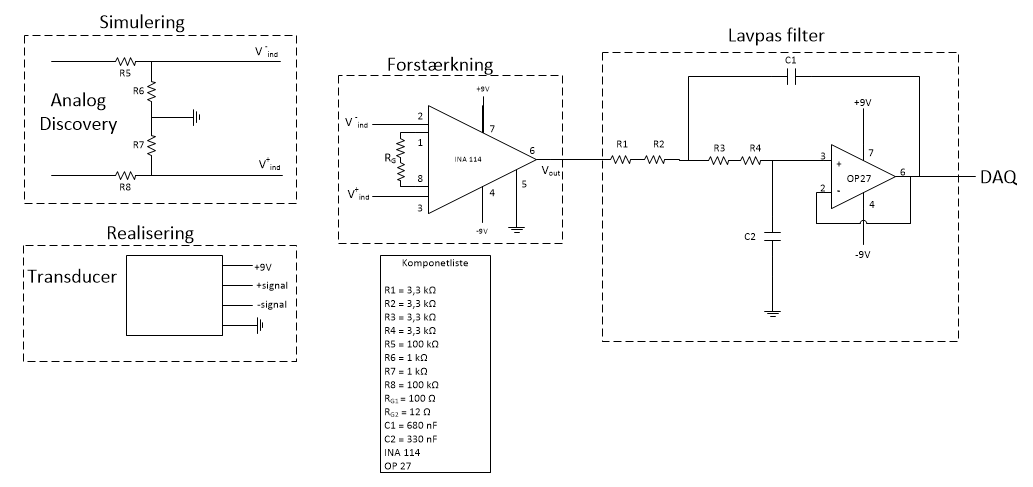
\includegraphics[width=1.0\textwidth]{Figurer/diagram_over_HW}
	\caption{Diagram over HW}
	\label{fig:HW}
\end{figure}

\subsubsection{Lavpas}
For at opnå den ønskede effekt i lavpasfilteret, blev det oplyst at $ f_c=50$ Hz, $ f_s = 1$kHz, $ R_1 = R_2 $ og $ C_2=680 nF$. Ud fra det udregnes de resterende komponentværdier for filteret.
  


\subsection{Modultest}
\subsubsection{Forstærkning}
\subsubsection{Lavpas}
For at teste lavpasfilteret foretages målinger med en sinus, hvor frekvensen variere for hver måling. Derved aflæses fasen, mellem indgang- og udgangssignal, og amplituden for hver måling. 
Ved knækfrekvensen skal fasedrejningen være 90\textdegree. Amplituden skal ændre sig XXX. Dette kan aflæses på billedet Måling for 50 Hz.
Efter knækfrekvensen skal amplituden blive mindre og mindre(går mod nul). På Måling for 60 Hz, kan det ses hvordan amplituden er faldet drastisk efter knækfrekvensen.  \\
\begin{figure}[H]
	\centering
	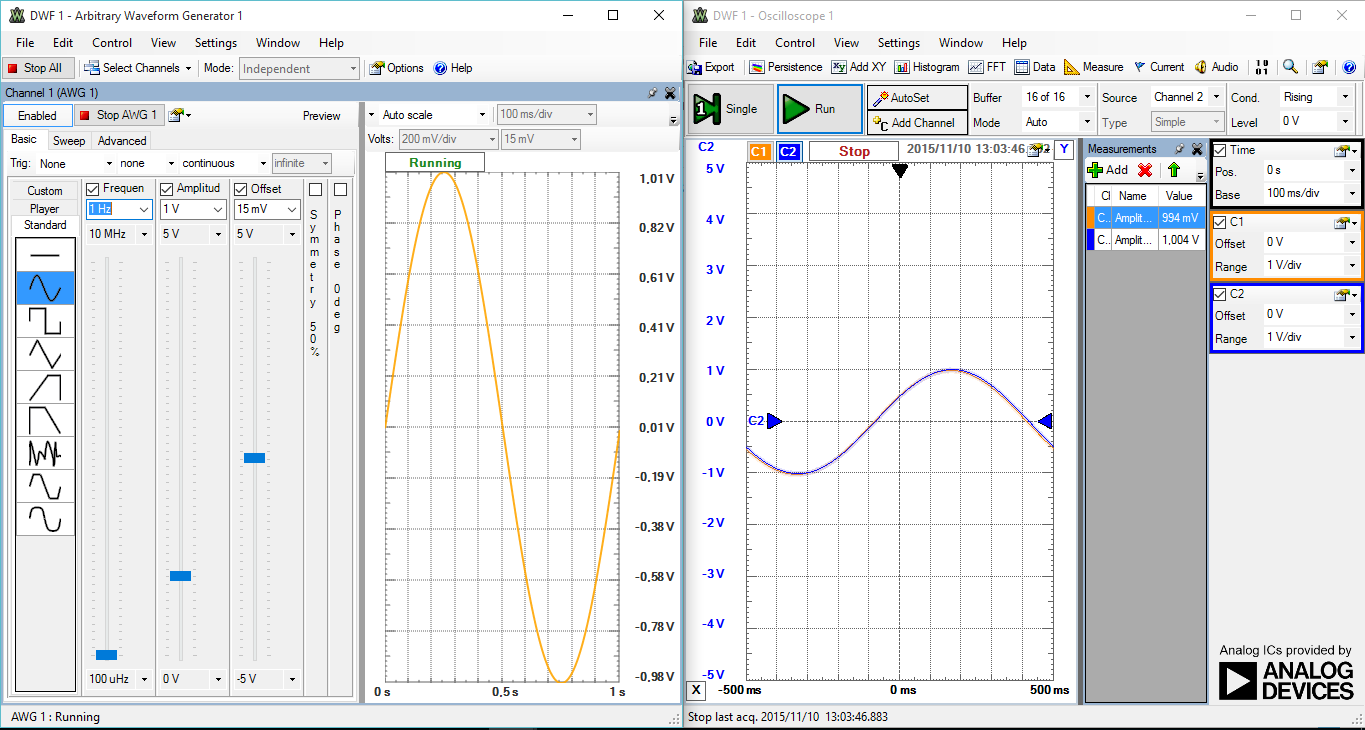
\includegraphics[width=1.0\textwidth]{Figurer/10Hz}
	\caption{Måling for 10 Hz}
	\label{fig:maeling10Hz}
\end{figure}

\begin{figure}[H]
	\centering
	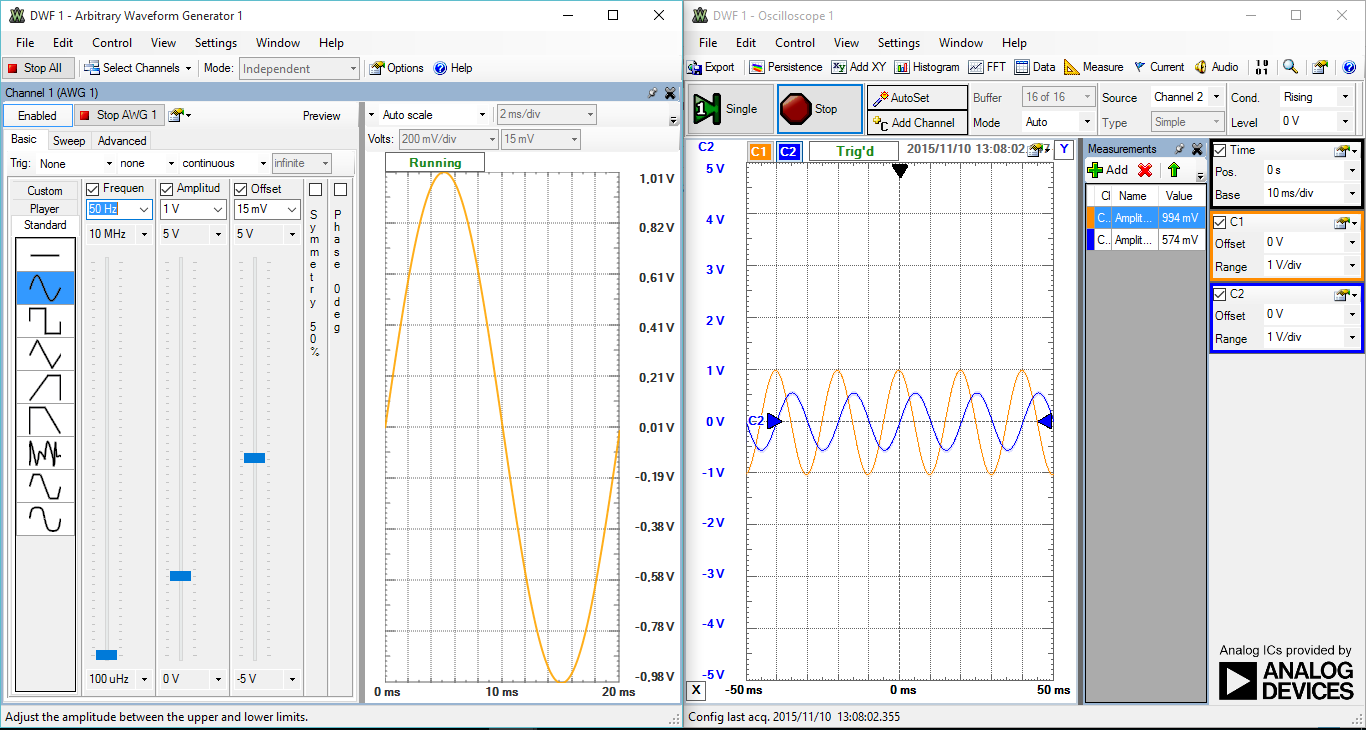
\includegraphics[width=1.0\textwidth]{Figurer/50Hz}
	\caption{Måling for 50 Hz}
	\label{fig:maeling50Hz}
\end{figure}

\begin{figure}[H]
	\centering
	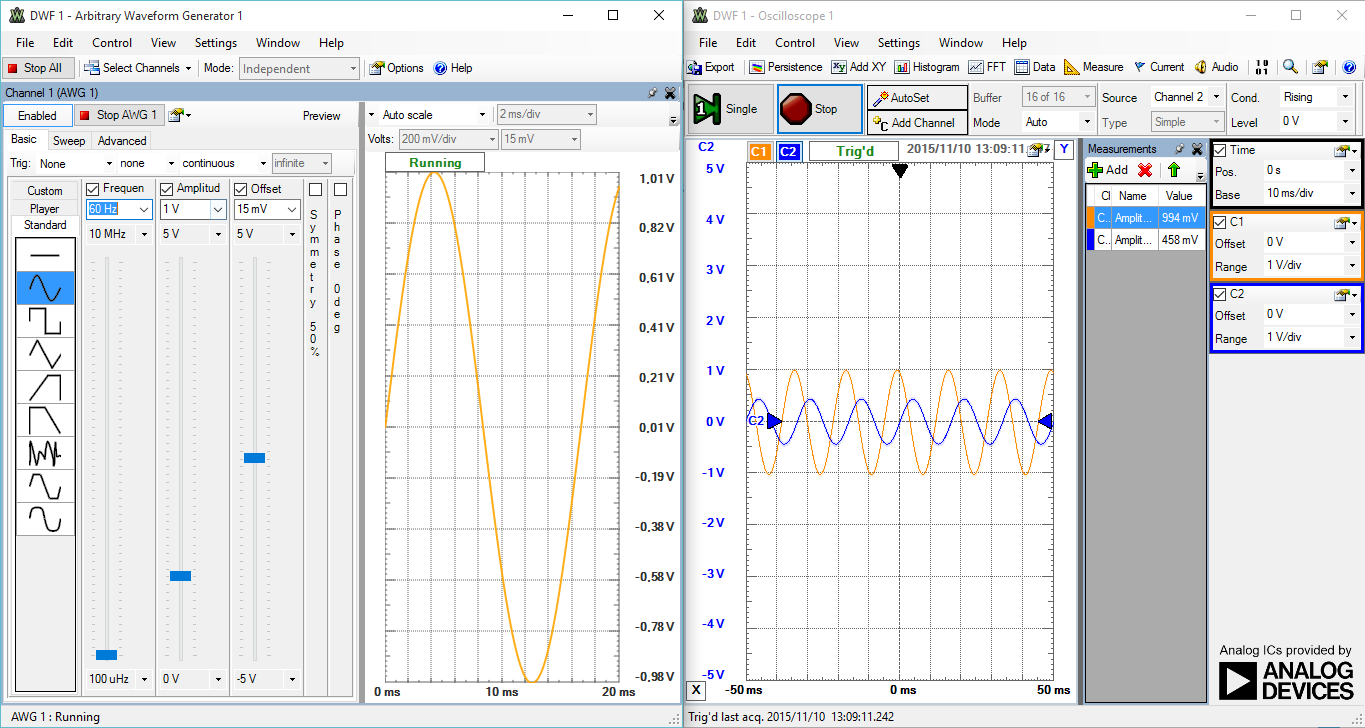
\includegraphics[width=1.0\textwidth]{Figurer/60Hz}
	\caption{Måling for 60 Hz}
	\label{fig:maeling60Hz}
\end{figure}

\subsubsection{Kalibrering med vandsøjle}
Efter forstærkning og lavpas er blevet testet hver for sig, udføres en kalibrering ved en vandsøjle. Her bruges en udleveret vandsøjle med tre målepunkter, hvor det er angivet hvor højt trykket er ved hver, i millimeter kviksølv. Derved kan det testes om hareware-delen måler den rigtige spænding i forhold til millimeter kviksølv. Ud fra den maksimale spænding og millimeter kviksølv kan det udregnes, hvad hardware skal vise ved 100 mmHg. 
\begin{figure}[H]
	\centering
	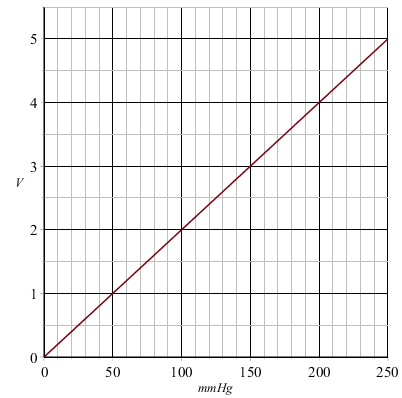
\includegraphics[width=0.3\textwidth]{Figurer/graf_vandtest}
	\caption{Graf til kalibrering, fra udregninger}
	\label{fig:graf_vandtest}
\end{figure}
Testen udføres ved, at der fyldes vand i søjlen til et bestemt punkt. Transduceren skal være tilkoblet et af de tre målepunkter, mens de andre er lukket til. Transduceren er sat til forstærkningen, der hvor Analog Discovery tidligere har været sat til. Transduceren er tilkoblet 0-9V, ved batterierne. På samme måde som ved simuleringen aflæses målingen på computeren ved hjælp af programmet WaveForms. Da det vides hvilken trykændring der måles på, ved vi fra grafen til kalibreringen, hvilken spænding den skal vise. Dette fortages for de tre målepunkter på vand søjlen, hvor hver måling sammenlignes med den udregnet graf. For hver gang, skal transduceren flyttes til et af de andre målepunkter.  
\begin{figure}[H]
	\centering
	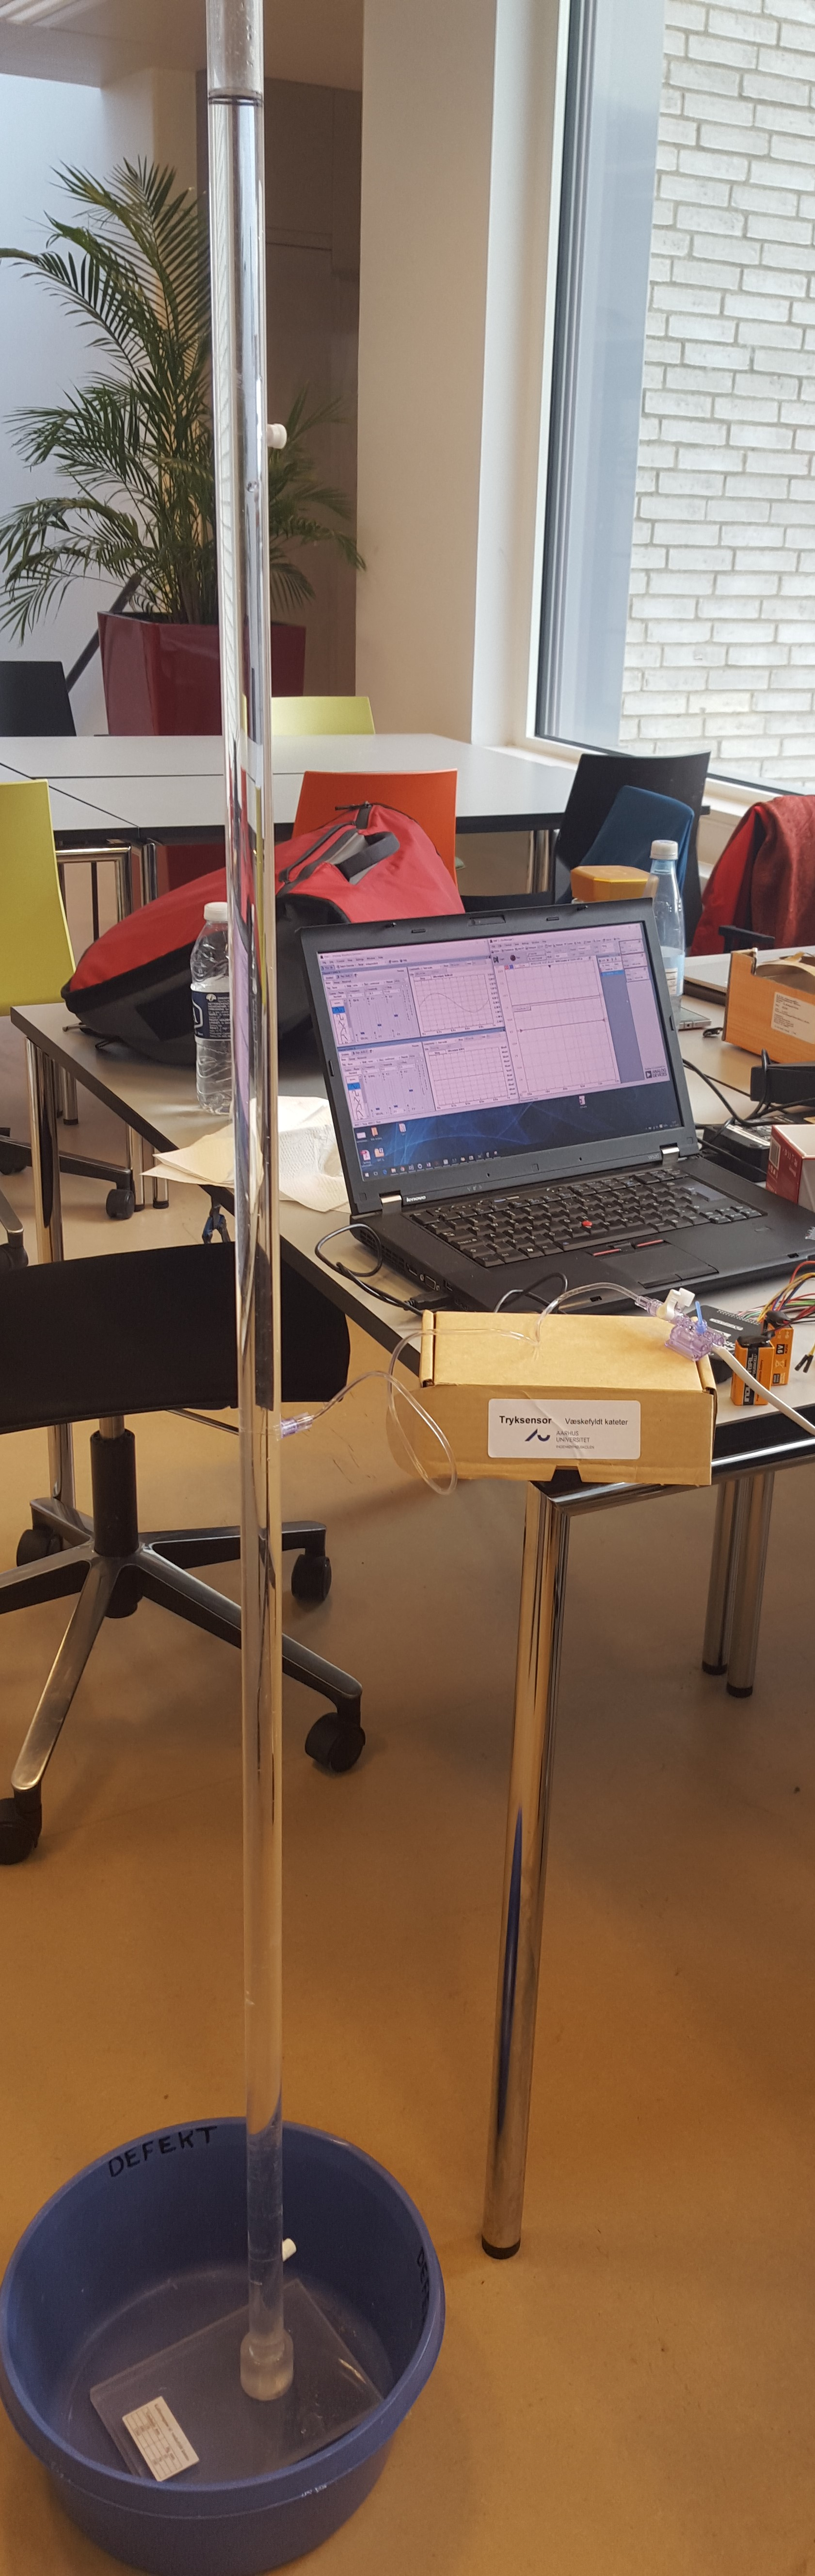
\includegraphics[width=0.2\textwidth]{Figurer/vandtest3}
	\caption{Opstilling}
	\label{fig:vandtest}
\end{figure} 
Test resultater.. 
\begin{figure}[H]
	\centering	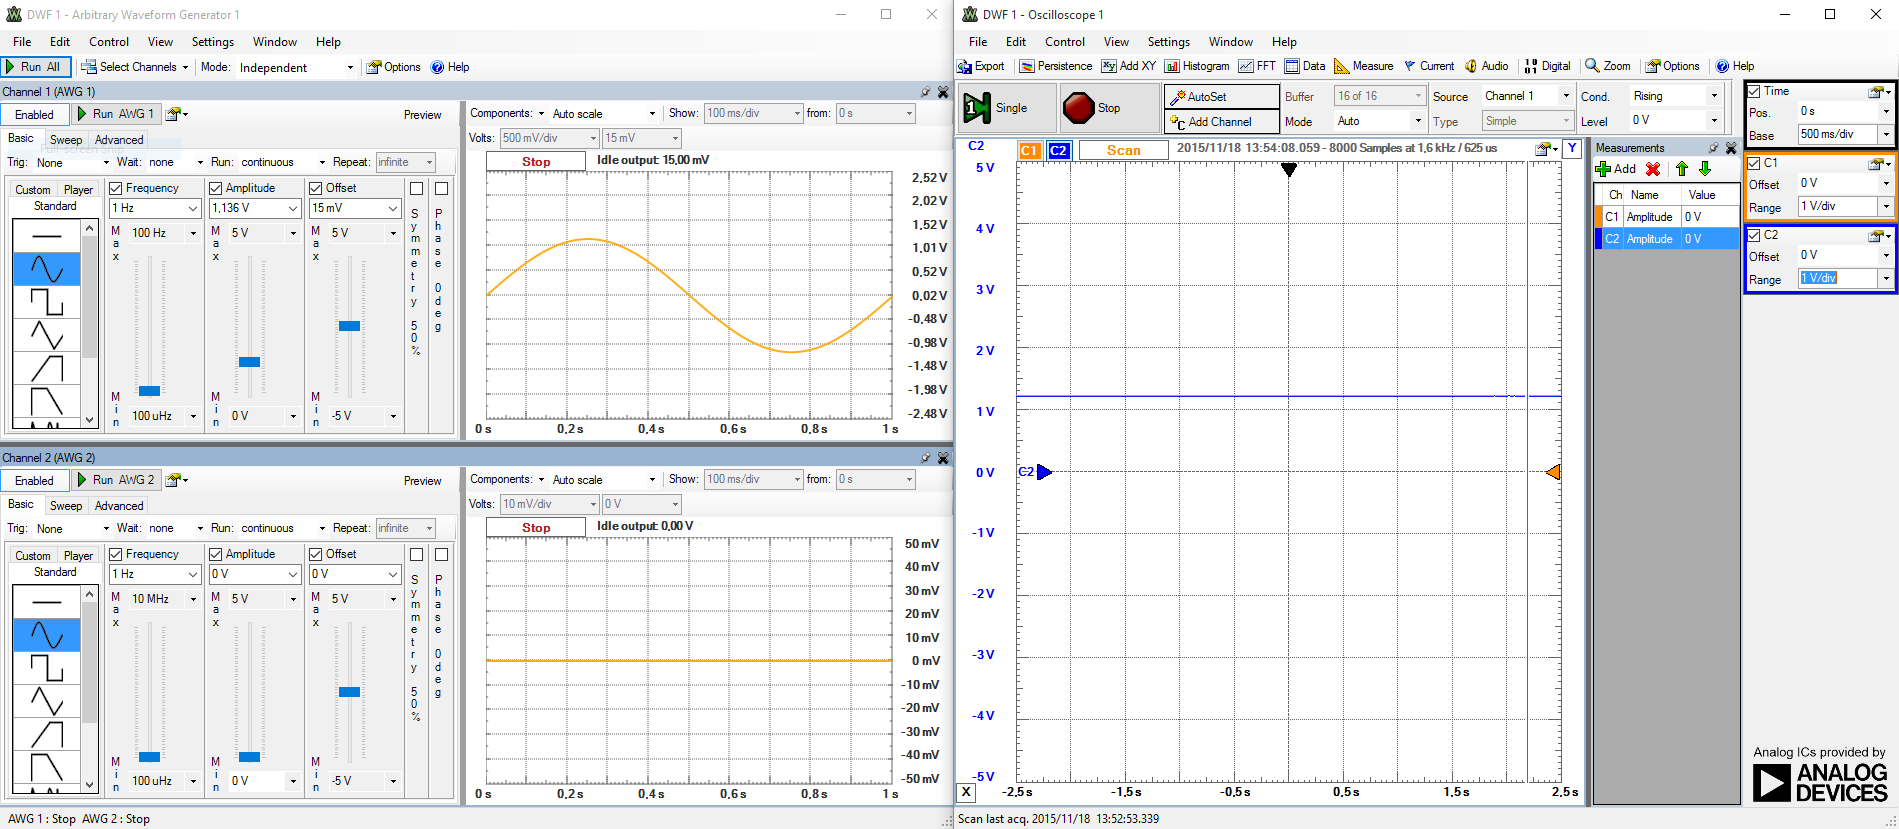
\includegraphics[width=1.0\textwidth]{Figurer/vandtest}
	\caption{Måling}
	\label{fig:vandtest_måling}
\end{figure} 


\section{Software}
\subsection{Design}
I dette beskrives systemets softwaredesign på baggrund af systembeskrivelsen og kravspecifikationen. De overvejelser vi har gjort i forbindelse med design og implementering af software vil blive præsenteret i dette afsnit. 

\subsubsection{Overordnet sekvensdiagram}
Overordnet set ønskes det at udvikle et system, der kan interagerer med en forsker. Diagrammet herunder viser at forskerens opgave består i at starte, tage stilling til nulpunktsjustering og kalibrering samt gemme de ønskede data. Diagrammet er en simpel illustration som viser systemets adfærd gennem alle fem Use Cases. Formålet med dette diagram er udelukkende at skabe et overblik over det samlede system.

\begin{figure}[H]
	\centering
	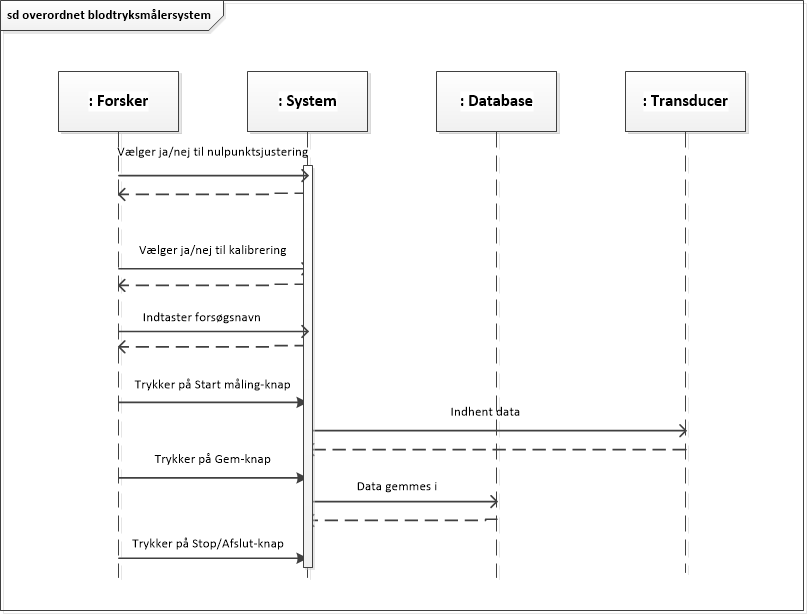
\includegraphics[width=0.7\textwidth]{Figurer/OverordnetSD}
	\caption{Overordnet sekvensdiagram for systemet}
	%\label{fig:Overordnet sekvensdiagram for systemet}
\end{figure}

\subsubsection{Problemidentifikation}
Første step i software designet er at klarlægge hvilke klasser systemet skal bestå af. Til dette er en domænemodel derfor udarbejdet med udgangspunkt i de fem Use Cases. I de fem Use Cases er de konceptuelle klasser blevet identificeret, og derefter indført som klasser i nedestående domænemodel. Modellen har til formål at vise hvilke dele systemet skal holde styr på. 

\begin{figure}[H]
	\centering
	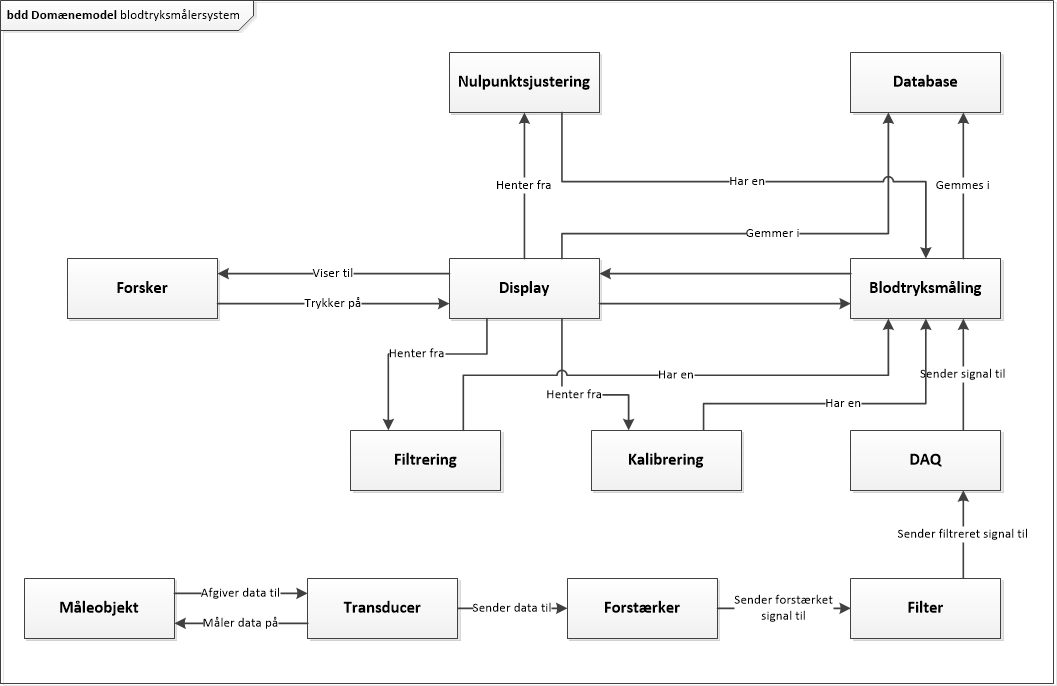
\includegraphics[width=1.0\textwidth]{Figurer/DomaneModel}
	\caption{Domænemodel}
	%\label{fig:Domænemodel}
\end{figure}

Diagrammet viser tydeligt forskerens interaktion med display, samt hvilke handlinger denne interaktion starter i system. Hardware-komponenterne er medtaget for at vise signalets vej fra måleobjekt til system. 

\subsubsection{Klasseidentifikation}
Ud fra domænemodellen kan et klassediagram udarbejdes, således tager dette diagram også udgangspunkt i de fem Use Cases. Hensigten med et klassediagram er at klarlægge hver klasses individuelle formål. 

\begin{figure}[H]
	\centering
	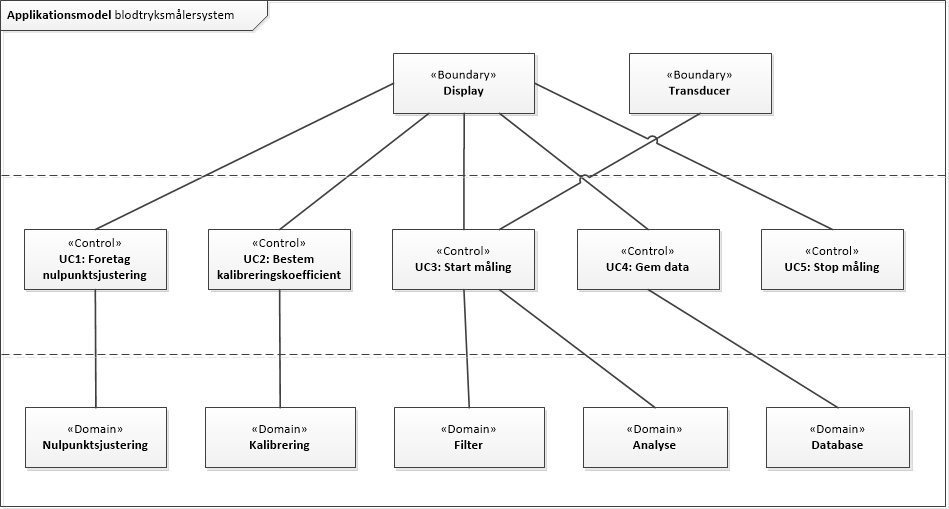
\includegraphics[width=1.0\textwidth]{Figurer/Applikationsmodel}
	\caption{Applikationsmodel for software}
	%\label{fig:Applikationsmodellen viser software klasser}
\end{figure}

Dermed ses det at denne model er delt op i tre niveauer:
\begin{enumerate}
\item Grænsefladeklasse
\begin{enumerate}
\item Transducer - Indhentet data fra måleobjekt
\item Display - Brugergrænseflade til forsker
\end{enumerate}
\item Kontrolklasse
\begin{enumerate}
\item UC1: Foretag nulpunktsjustering
\item UC2: Foretag kalibrering
\item UC3: Start måling
\item UC4: Gem måling
\item UC5: Afslut måling
\end{enumerate}
\item Domæneklasse
\begin{enumerate}
\item Database
\end{enumerate}
\end{enumerate}

\subsubsection{Metodeidentifikation}
Klasserne i ovenstående klassediagram er med til at definere, hvilke blokke de følgende sekvensdiagrammer må indeholde. Det er yderst vigtigt at der er en sammenhæng mellem klasserne i klassediagrammet og blokkene i sekvensdiagrammet. Vi har valgt at udarbejde et sekvensdiagram for hver enkelt Use Case, hvori systemets interne kommunikation beskrives, når både normalforløb og undtagelser gennemløbes. I alle diagrammerne beskrives forløbet via de metodekald, der er nødvendige for at få de ønskede handlinger mellem blokkene udført. 

\textbf{Use Case 1}
\begin{figure}[H]
	\centering
	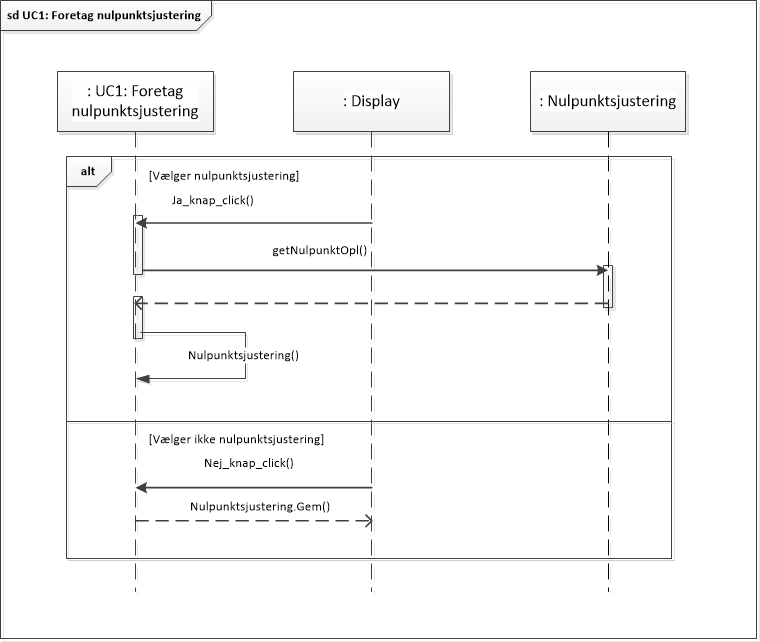
\includegraphics[width=0.7\textwidth]{Figurer/UC1}
	\caption{Sekvensdiagram for Use Case 1}
	%\label{fig:Sekvensdiagram for Use Case 1 - Foretag nulpunktsjustering}
\end{figure}
Det ses af ovenstående sekvensdiagram at forsker interagerer med display. Her er der to mulige udfald "Vælger nulpunktsjustering" og "Vælger ikke nulpunktsjustering", disse implementeres som to muligheder forsker kan vælge imellem. 

\textbf{Use Case 2}
\begin{figure}[H]
	\centering
	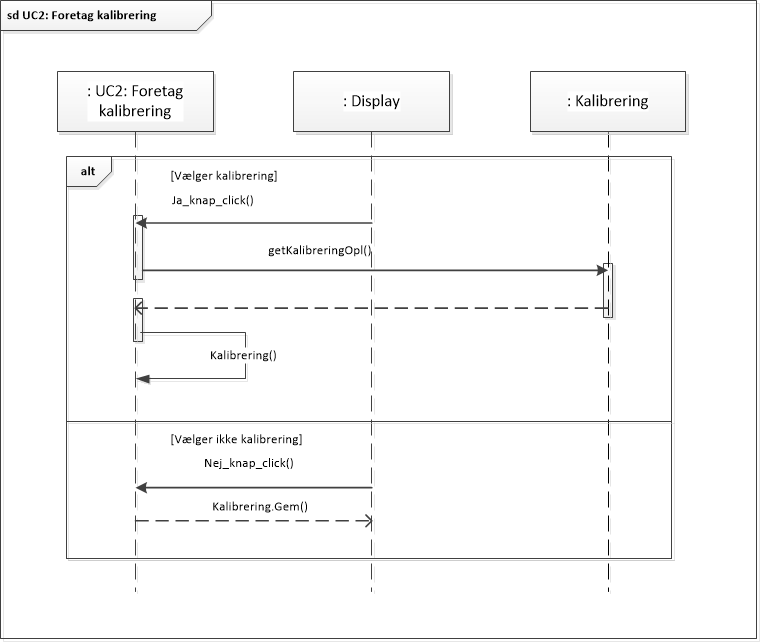
\includegraphics[width=0.7\textwidth]{Figurer/UC2}
	\caption{Sekvensdiagram for Use Case 2}
	%\label{fig:Sekvensdiagram for Use Case 2 - Foretag kalibrering}
\end{figure}
Diagrammet ovenfor viser at forsker interagerer med display, hvor der ved tryk enten vælges ja eller nej til kalibering. Afhængig af valg foretager systemet de nødvendige kald.

\textbf{Use Case 3}
\begin{figure}[H]
	\centering
	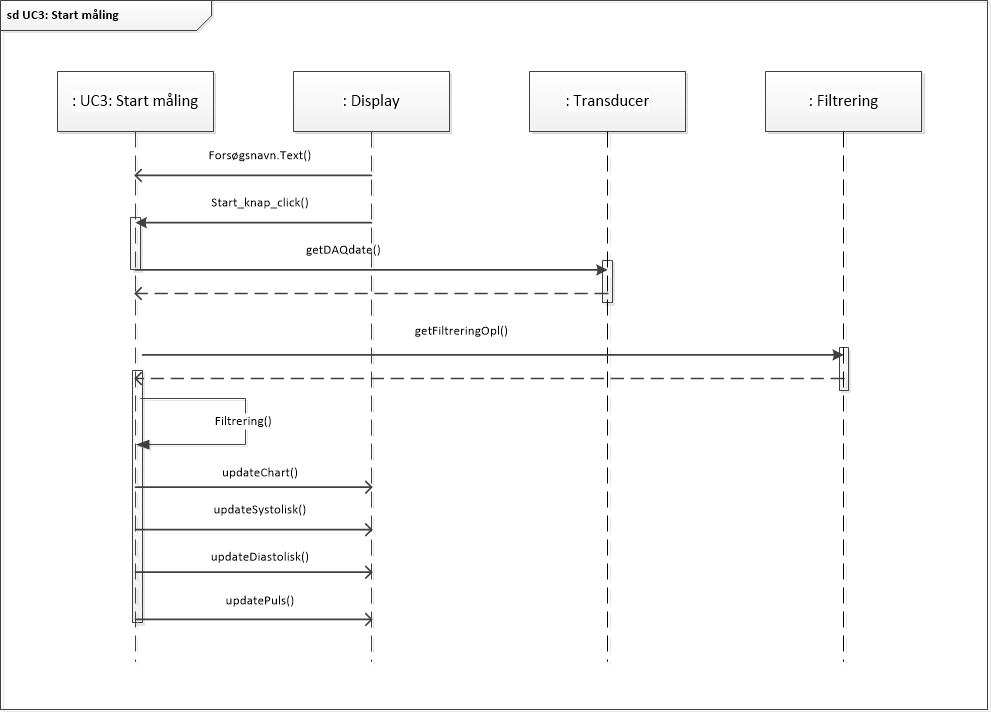
\includegraphics[width=0.7\textwidth]{Figurer/UC3}
	\caption{Sekvensdiagram for Use Case 3}
	%\label{fig:Sekvensdiagram for Use Case 3 - Start måling}
\end{figure}
Ved Use Case 3 - Start måling ses det at display, transducer og filtreringsklassen vil komme i spil. Her modtages besked ved indtastning af forsøgsnavn og tryk på start-knap på display om, at signaldata fra transduceren skal hentes ind i systemet. Herefter foretages filtrering af signalet, samt visning af signal i graf, systoliske-, diastoliske og puls-værdier på display. Use Casen indeholder en undtagelse hvor filtrering af signal ikke ønskes foretaget, denne er ikke medtaget i sekvensdiagrammet.

\textbf{Use Case 4}
\begin{figure}[H]
	\centering
	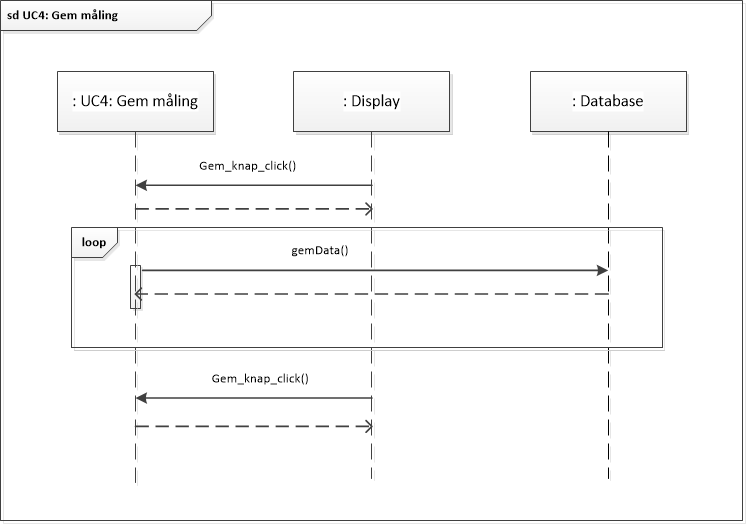
\includegraphics[width=0.7\textwidth]{Figurer/UC4}
	\caption{Sekvensdiagram for Use Case 4}
	%\label{fig:Sekvensdiagram for Use Case 4 - Gem data}
\end{figure}
Ovenstående diagram viser at for at få gemt data fra signalet, kræver det at der trykkes på Gem-knap på display, hvor efter systemet konstant vil sende data ned i databasen indtil der igen trykkes på Gem-knappen, for at stoppe gemning af data. 

\textbf{Use Case 5}
\begin{figure}[H]
	\centering
	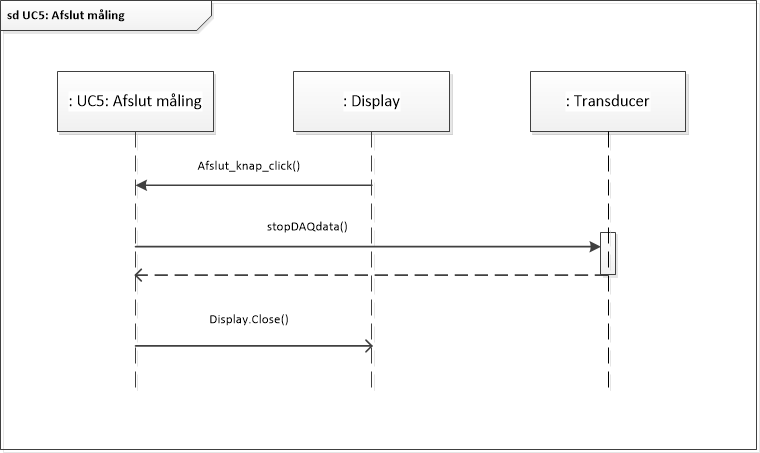
\includegraphics[width=0.7\textwidth]{Figurer/UC5}
	\caption{Sekvensdiagram for Use Case 5}
	%\label{fig:Sekvensdiagram for Use Case 5 - Afslut måking}
\end{figure}
Ved afslutning af en måling ses det at forsker trykker på Afslut-knap på display, hvorefter indhentening af data fra DAQ stoppes og programmet lukker ned.

\subsection{Implementering}
\begin{enumerate}
\item Observer - strategy
\item Oprettelse af metoder - trelagsmodel
\item Forklar princippet bag kalibrering og nulpunktsjustering, beregningerne
\item Visning i graf
\item Bestemmelse af systolisk, diastolisk og puls 
\item GUI design
\item Aktivitetsdiagrammer
\item Klassediagrammer
\item Database
\end{enumerate}

\subsection{Modultest}
\begin{enumerate}
\item GUI test
\item Test af tråde (observer strategy)
\item Test af systolisk, diastolisk og puls-værdier
\item Test af Gem i database
\end{enumerate}